\section{Lösungsansatz}
\label{sec:Lösungsansatz}

Ziel dieses Projektes war es Wasser auf Satellitenbildern zu erkennen.
Dazu wurden zwei Methoden des maschinellen Lernens für die Segmentierung verwendet.
Ein \enquote{Convolutional Neural Network} stellte dabei die Hauptmethode dar 
und ein \enquote{Random Forest} stellte dabei eine Alternativmethode zum Vergleich dar.
Für beide Methoden wurde das Framework \enquote{TensorFlow} verwendet.\cite{tensorflow}
Die Metrik, die benutzt wurde um die Methoden zu evaluieren, war die Genauigkeit(zu englisch \enquote{accuracy}), 
also der Anteil der richtig zugeordneten Pixel.

\subsection{Vorverarbeitung}
\label{ssec:Vorverarbeitung}

Der in \autoref{sec:Datensatz} beschriebene Datensatz wurde in drei Teildatensätze aufgeteilt,
den Trainings-, den Validierungs- und den Testdatensatz.
Die Größen dieser Datensätze sind in \autoref{tab:Teildatensätze} angegeben.

\begin{table}
    \centering
    \caption{Größen der Teildatensätze vom Gesamtdatensatz mit 57931 Satellitenbildern.}
    \label{tab:Teildatensätze}
    \begin{tabular}{l c c c}
        \toprule 
        & Trainingsdaten & Validierungsdaten & Testdaten \\ 
        \midrule 
        Anzahl & 39392 & 6952 & 11587 \\
        Anteil & 68\% & 12\% & 20\% \\
        \bottomrule
    \end{tabular}
\end{table}

Außerdem wurden die Bilder zu einer Auflösung von 128 x 128 Pixel skaliert, 
da so nicht viel Information verloren ging und viel Rechenzeit und Rechenleistung eingespart werden konnte.
Die Pixel der Maskenbilder wurden zu binären Werten umgerechnet, wobei 1 Wasser und 0 kein Wasser kennzeichnet
und die drei Farbkanäle Satellitenbilder wurden auf einen Pixelwert zwischen 0 und 1 normiert. 

\subsection{Hauptmethode: \enquote{Convolutional Neural Network}}
\label{ssec:Hauptmethode}

Das verwendete Neuronale Netzwerk ist vollständig \enquote{convolutional} und orientiert sich an der häufig für Segmentierung verwendeten \enquote{U-Net}-Struktur.\cite{ronneberger2015unet}
Hier wird in der ersten Hälfte des Netzwerks zwischen den \enquote{convolutional} Lagen das Bild in durch maximales \enquote{Pooling} verkleinert (halbierte Kantenlänge) 
und in der zweiten Hälfte das Bild zwischen den \enquote{convolutional} Lagen durch transponierte \enquote{convolutional} Lagen vergrößert (verdoppelte Kantenlänge).
Zusätzlich wird die Ausgabe vor dem Verkleinern kopiert und mit der Ausgabe nach dem Vergrößern verkettet.
Ein Beispiel eines solchen \enquote{U-Net} ist in \autoref{fig:unet} dargestellt.

Allerdings unterscheidet sich das verwendete Netzwerk in einigen Hyperparametern, wie z.B. die Filteranzahlen und die Pixelanzahlen.
Außerdem wurde zwischen den beiden \enquote{convolutional} Lagen einer Ebene das Netzwerk mithilfe von \enquote{Dropout} regularisiert.
Ein weiterer Unterschied zum dargestellten \enquote{U-Net} ist, dass bei den \enquote{convolutional} Lagen ein \enquote{Padding} von \enquote{same} statt \enquote{valid} verwendet wurde.

Als Aktivierungsfunktion wurde für alle \enquote{convolutional} Lagen die \enquote{ReLU}-Funktion und für die letzte Lage die \enquote{Sigmoid}-Funktion verwendet.
Der Optimierer \enquote{Adam} hat dabei die Verlustfunktion der binären Kreuzentropie minimiert.

\begin{figure}
    \centering
    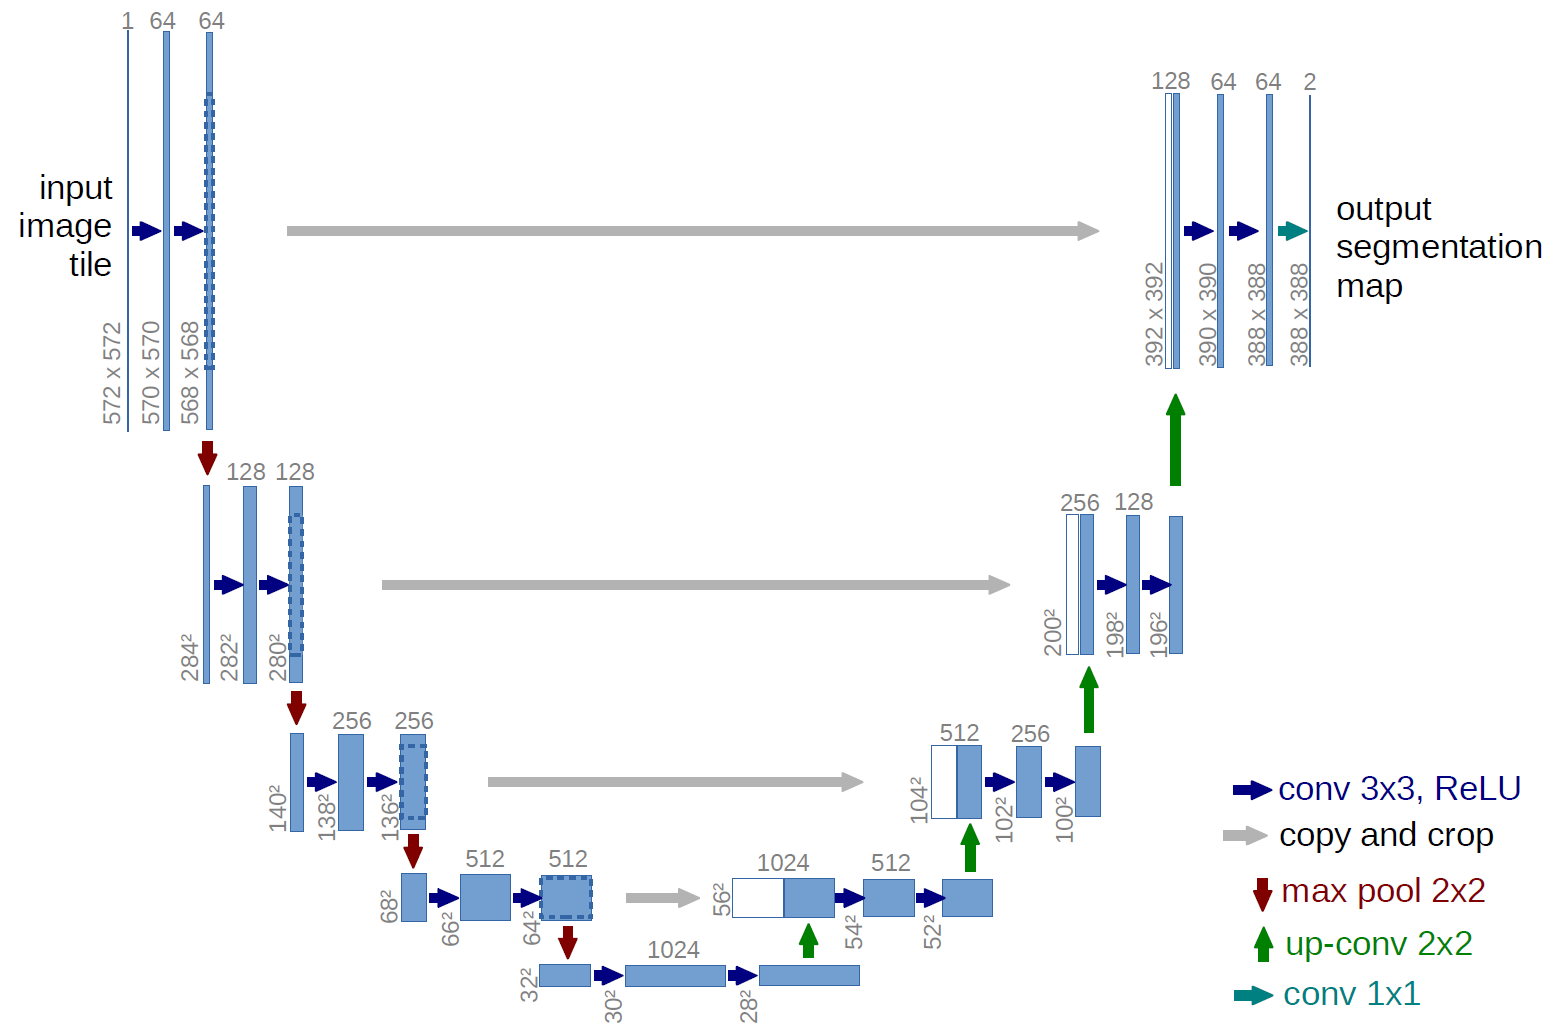
\includegraphics[width=0.6\textwidth]{images/unet.png}
    \caption{Visualisierung eines \enquote{U-Net}, %
    wobei jede Box einem Mehrkanal-Bild entspricht. Die Anzahl an Kanäle ist über der Box angegeben und die Anzahl der Pixel ist neben der Box angegeben. %
    Jeder Pfeil entspricht der entsprechenden Operation.\cite{ronneberger2015unet}}
    \label{fig:unet}
\end{figure}

Die besten Hyperparameter und die beste Struktur des Netzwerks wurde mithilfe einer zufälligen Gittersuche ermittelt.
Das Netzwerk wurde für 100 verschiedene Kombinationen der Hyperparameter auf einem kleinen Trainingsdatensatz von 3000 Satellitenbildern für 20 Epochen trainiert
und dann auf einem kleinen Validierungsdatensatz von ebenfalls 3000 Satellitenbildern evaluiert.
Das Ergebnis der Hyperparametersuche ist in \autoref{fig:grid_search} dargestellt und in \autoref{tab:grid_search} sind die besten fünf Kombinationen aufgelistet.
Vor dieser systematischen Suche wurden weitere Hyperparameter variiert, allerdings erwies sich das zuvor beschriebene Neuronale Netzwerk als am besten geeignet
und die systematischen Suche beschränkte sich auf die wichtigsten Parameter.
Variiert wurden folgende Hyperparameter:

\begin{itemize}
    \item \enquote{filter\_start}: Anzahl der Filter der \enquote{convolutional} Lagen der obersten Ebene, wobei die Filter pro Ebene verdoppelt wurden
    \item \enquote{filter\_levels}: Anzahl der Ebenen
    \item \enquote{kernel\_size}: Größe der Faltungsmatrizen aller \enquote{convolutional} Lagen
    \item \enquote{kernel\_initializer}: Methode der Matrixinitialisierung aller \enquote{convolutional} Lagen
    \item \enquote{dropout\_start}: Stärke des \enquote{Dropout} der obersten Ebene, wobei die Stärke jeweils nach zwei Ebenen um 0,1 erhöht wurde
    \item \enquote{learning\_rate}: Lernrate des verwendeten Optimierers \enquote{Adam}
\end{itemize}

\begin{figure}
    \centering
    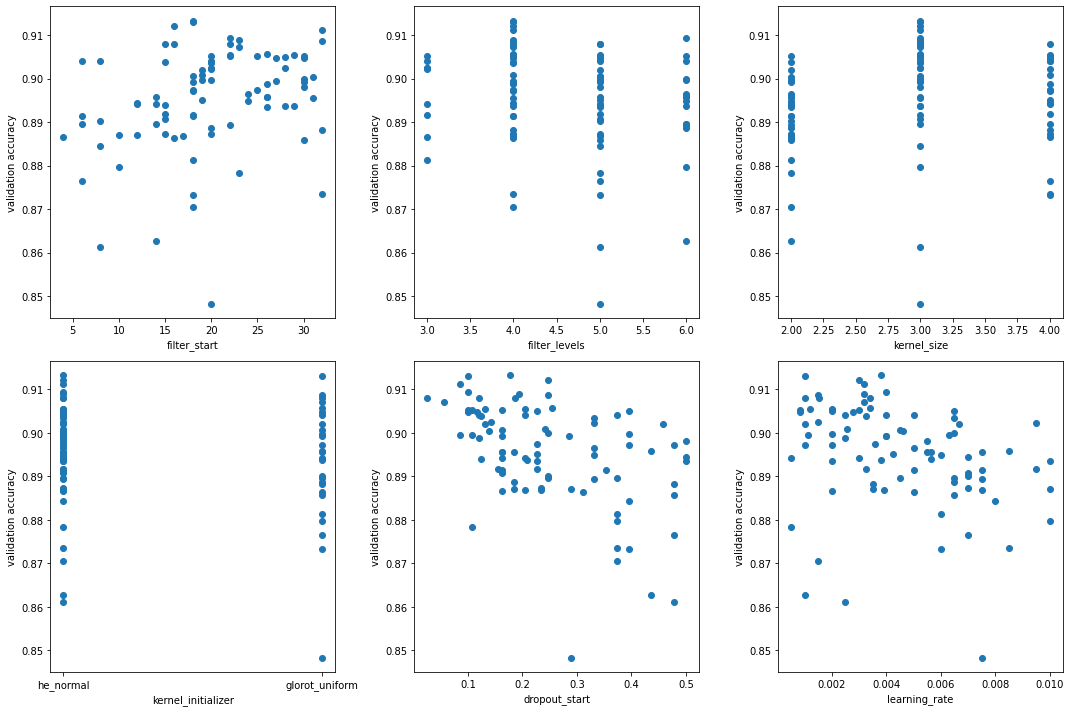
\includegraphics[width=0.8\textwidth]{images/grid_search.png}
    \caption{Zufällige Suche der besten Hyperparameter}
    \label{fig:grid_search}
\end{figure}

\begin{table}
    \centering
    \caption{Die besten fünf Ergebnisse der zufälligen Gittersuche mit der Genauigkeit auf den 3000 Testdaten und den zugehörigen Hyperparametern}
    \label{tab:grid_search}
    \resizebox{\textwidth}{!}{%
    \begin{tabular}{c c c c c c c}
        \toprule
        Genauigkeit & \enquote{filter\_start} & \enquote{filter\_levels} & \enquote{kernel\_size} & \enquote{kernel\_initializer} & \enquote{dropout\_start} & \enquote{learning\_rate} \\
        \midrule
        0.913355 & 18 & 4 & 3 & he\_normal & 0.177895 & 0.003795 \\
        0.913100 & 18 & 4 & 3 & glorot\_uniform & 0.100000 & 0.001000 \\
        0.912037 & 16 & 4 & 3 & he\_normal & 0.247368 & 0.003000 \\
        0.911288 & 32 & 4 & 3 & he\_normal & 0.086316 & 0.003179 \\
        0.909450 & 22 & 6 & 3 & he\_normal & 0.100000 & 0.004000 \\
        \bottomrule
    \end{tabular}%
    }
\end{table}

Aus der Suche ergab sich eine Kombination mit der besten Genauigkeit von 91,33\% auf dem Testdatensatz.
Das dadurch entstandene Netzwerk wurde dann für den gesamten Datensatz verwendet und wird im Anhang anhand einer Visualisierung detailliert beschrieben. (siehe \autoref{fig:visual_model})

Der Fortschritt während des Trainings der 50 Epochen ist in \autoref{fig:train_hist} dargestellt.
Hier lässt sich erkennen, dass das Modell etwas besser auf den Trainingsdaten abschneidet, aber eine Überanpassung ist dies nicht.
Bei fast 40000 Bildern mit einer Auflösung von 128 x 128 Pixel und so unterschiedlichen Bildern ist eine Überanpassung nicht möglich 
und ein niedriger Dropout wie hier reicht für die Regularisierung aus.
Die Hyperparametersuche zeigte auch, dass ein zu hoher Dropout nur zu schlechteren Ergebnissen führte.
Die \enquote{Zackigkeit} der Kurven in \autoref{fig:train_hist} lässt sich dadurch erklären, dass eine \enquote{Batch}-Größe von 128 Bildern verwendet wurde und ein großer Teil des Trainings so gar nicht in den Plots zu erkennen ist.
Eine Erhöhung der Epochenanzahl war aufgrund von fehlenden Rechenkapazitäten nicht möglich.

\begin{figure}
    \centering
    \begin{subfigure}{0.45\textwidth}
        \centering
        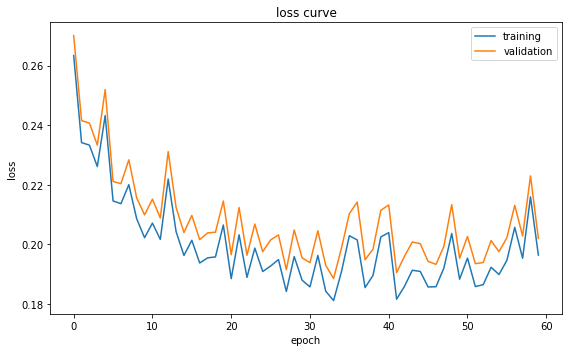
\includegraphics[width=\textwidth]{images/loss_curve.png}
        \caption{Verlustfunktion}
        \label{fig:loss_curve}
    \end{subfigure}
    \begin{subfigure}{0.45\textwidth}
        \centering
        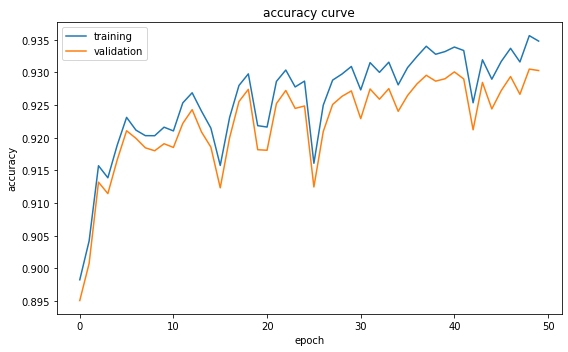
\includegraphics[width=\textwidth]{images/acc_curve.png}
        \caption{Genauigkeit}
        \label{fig:acc_curve}
    \end{subfigure}
    \caption{Plots der Verlustfunktion bzw. Genauigkeit während dem Training je nach Epoche auf Trainings- und Validierungsdatensatz}
    \label{fig:train_hist}
\end{figure}

Da die Pixel der Ausgabebilder des Netzwerks Werte zwischen 0 und 1 annimmt, wurde die Genauigkeit auf dem Validierungsdatensatz
für verschiedene Schwellwerte berechnet, ab denen ein Pixel als Wasser gewertet wird und der beste Schwellwert wird verwendet.
Hier ergab sich als bester Schwellwert 0,54.
Dies ist in \autoref{fig:threshold} dargestellt.

\begin{figure}
    \centering
    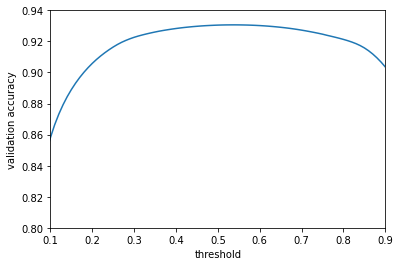
\includegraphics[width=0.4\textwidth]{images/threshold.png}
    \caption{Plot der Genauigkeit auf dem Validierungsdatensatz gegen den Schwellwert}
    \label{fig:threshold}
\end{figure}

\subsection{Alternativmethode: \enquote{Random Forest}}
\label{ssec:Alternativmethode}

Zum Vergleich mit dem Neuronalen Netzwerks wurde eine pixelweise Klassifizierung mithilfe eines \enquote{Random Forest} verwendet.
Auch hierfür wurde das Framework \enquote{TensorFlow} verwendet, allerdings wurde dies um das Framework \enquote{TensorFlow Decision Forests} erweitert.\cite{tfdf}
Dieser \enquote{Random Forest} besteht aus 60 Entscheidungsbäumen, die eine maximale Tiefe von 32 haben.

Hierfür wurden zunächst jedem Pixel der Satellitenbilder einige Attribute extrahiert.
Auf jedem Farbkanal wurde der Betrag des Gradienten berechnet.
Dann wurde vom Satellitenbild und dem Bild der Gradienten ein Graustufen Bild erzeugt.
All diese 8 Attribute wurden dem \enquote{Random Forest} pixelweise übergeben.

Aufgrund von Arbeitsspeicher- und Rechenzeit-Limitierungen konnte nicht der gesamte Trainingsdatensatz verwendet werden.
Aus jedem Bild im Trainingsdatensatz wurden 25 zufällige Pixel verwendet und so wurde der \enquote{Random Forest} auf etwa einer Millionen Pixel trainiert.
Der Validierungs- und Testdatensatz blieb jedoch gleich.
